\section{Inference Ensemble}

The deployment of the recommendation system in inference mode involves setting up the Triton Ensemble and the external components of the system as shown bellow in Figure \ref{fig:DeploymentDiagram}.

\begin{figure}[H]
    \centering
    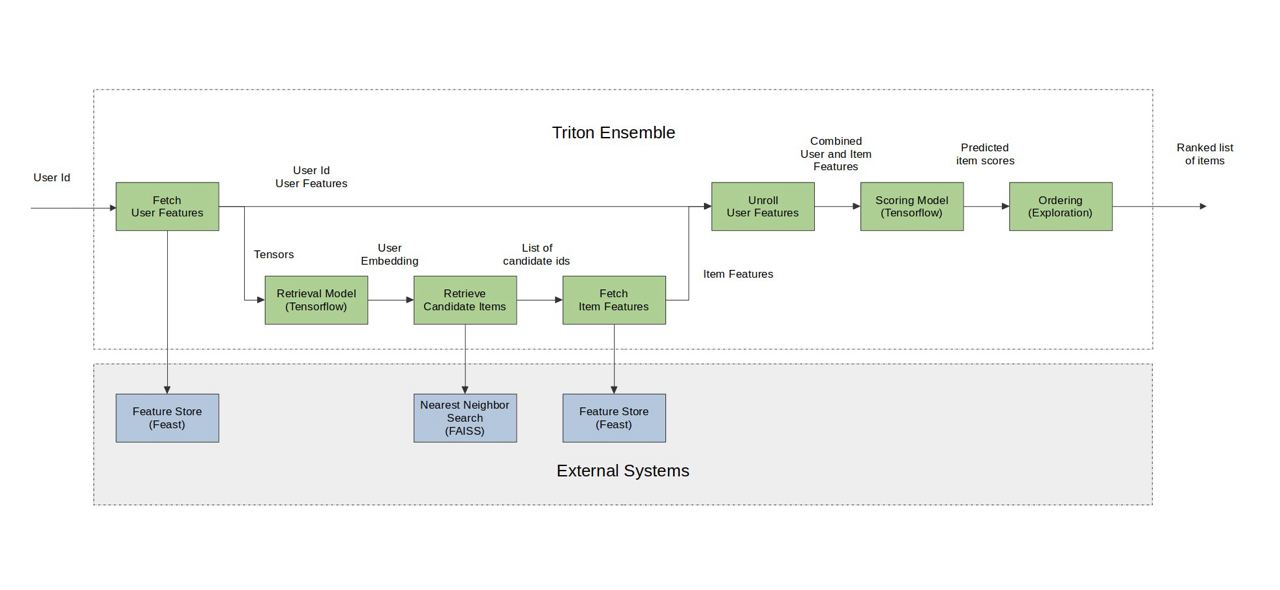
\includegraphics[width=\textwidth]{assets/deployment.jpg}
    \caption{Inference Ensemble Diagram}
    \label{fig:DeploymentDiagram}
\end{figure}

Initially, the ensemble receives a user ID as input. Once received, Triton starts executing the ensemble pipeline step by step, which consists of the following steps:

\subsubsection{Fetch User Features}

In this step, the server fetches the user features from the feature store (Feast). Then those features are processed by the workflow that was defined previously and saved in the model repository.

\subsubsection{Generate User Embedding}

Once the server has the user features, it uses them to generate a user embedding. 
It loads the query tower of the retrieval model, which is responsible for generating the user embedding. 

\subsubsection{Retrieve Candidate Item IDs}

After generating the user embedding, the server uses it to retrieve a list of candidate item IDs through a nearest neighbor search. 
The server uses FAISS \cite{Faiss} to perform the nearest neighbor search computation on a GPU.
Faiss returns a list of candidate item IDs based on their embedding similarity to the user embedding.

\subsubsection{Fetch Item Features}

The server fetches the item features from the feature store (Feast) based on the candidate item IDs retrieved in the previous step.
And feeds those features into the pre-processing workflow that was defined previously and saved in the model repository.

\subsubsection{Unroll User Features}

After fetching the item features, the server combines them with the user features using an operation called "Unrolling", where the user features are repeated for each item in the candidate list as shown in Figure \ref{fig: UnrollUserFeatures}.

\begin{figure}[H]
    \centering
    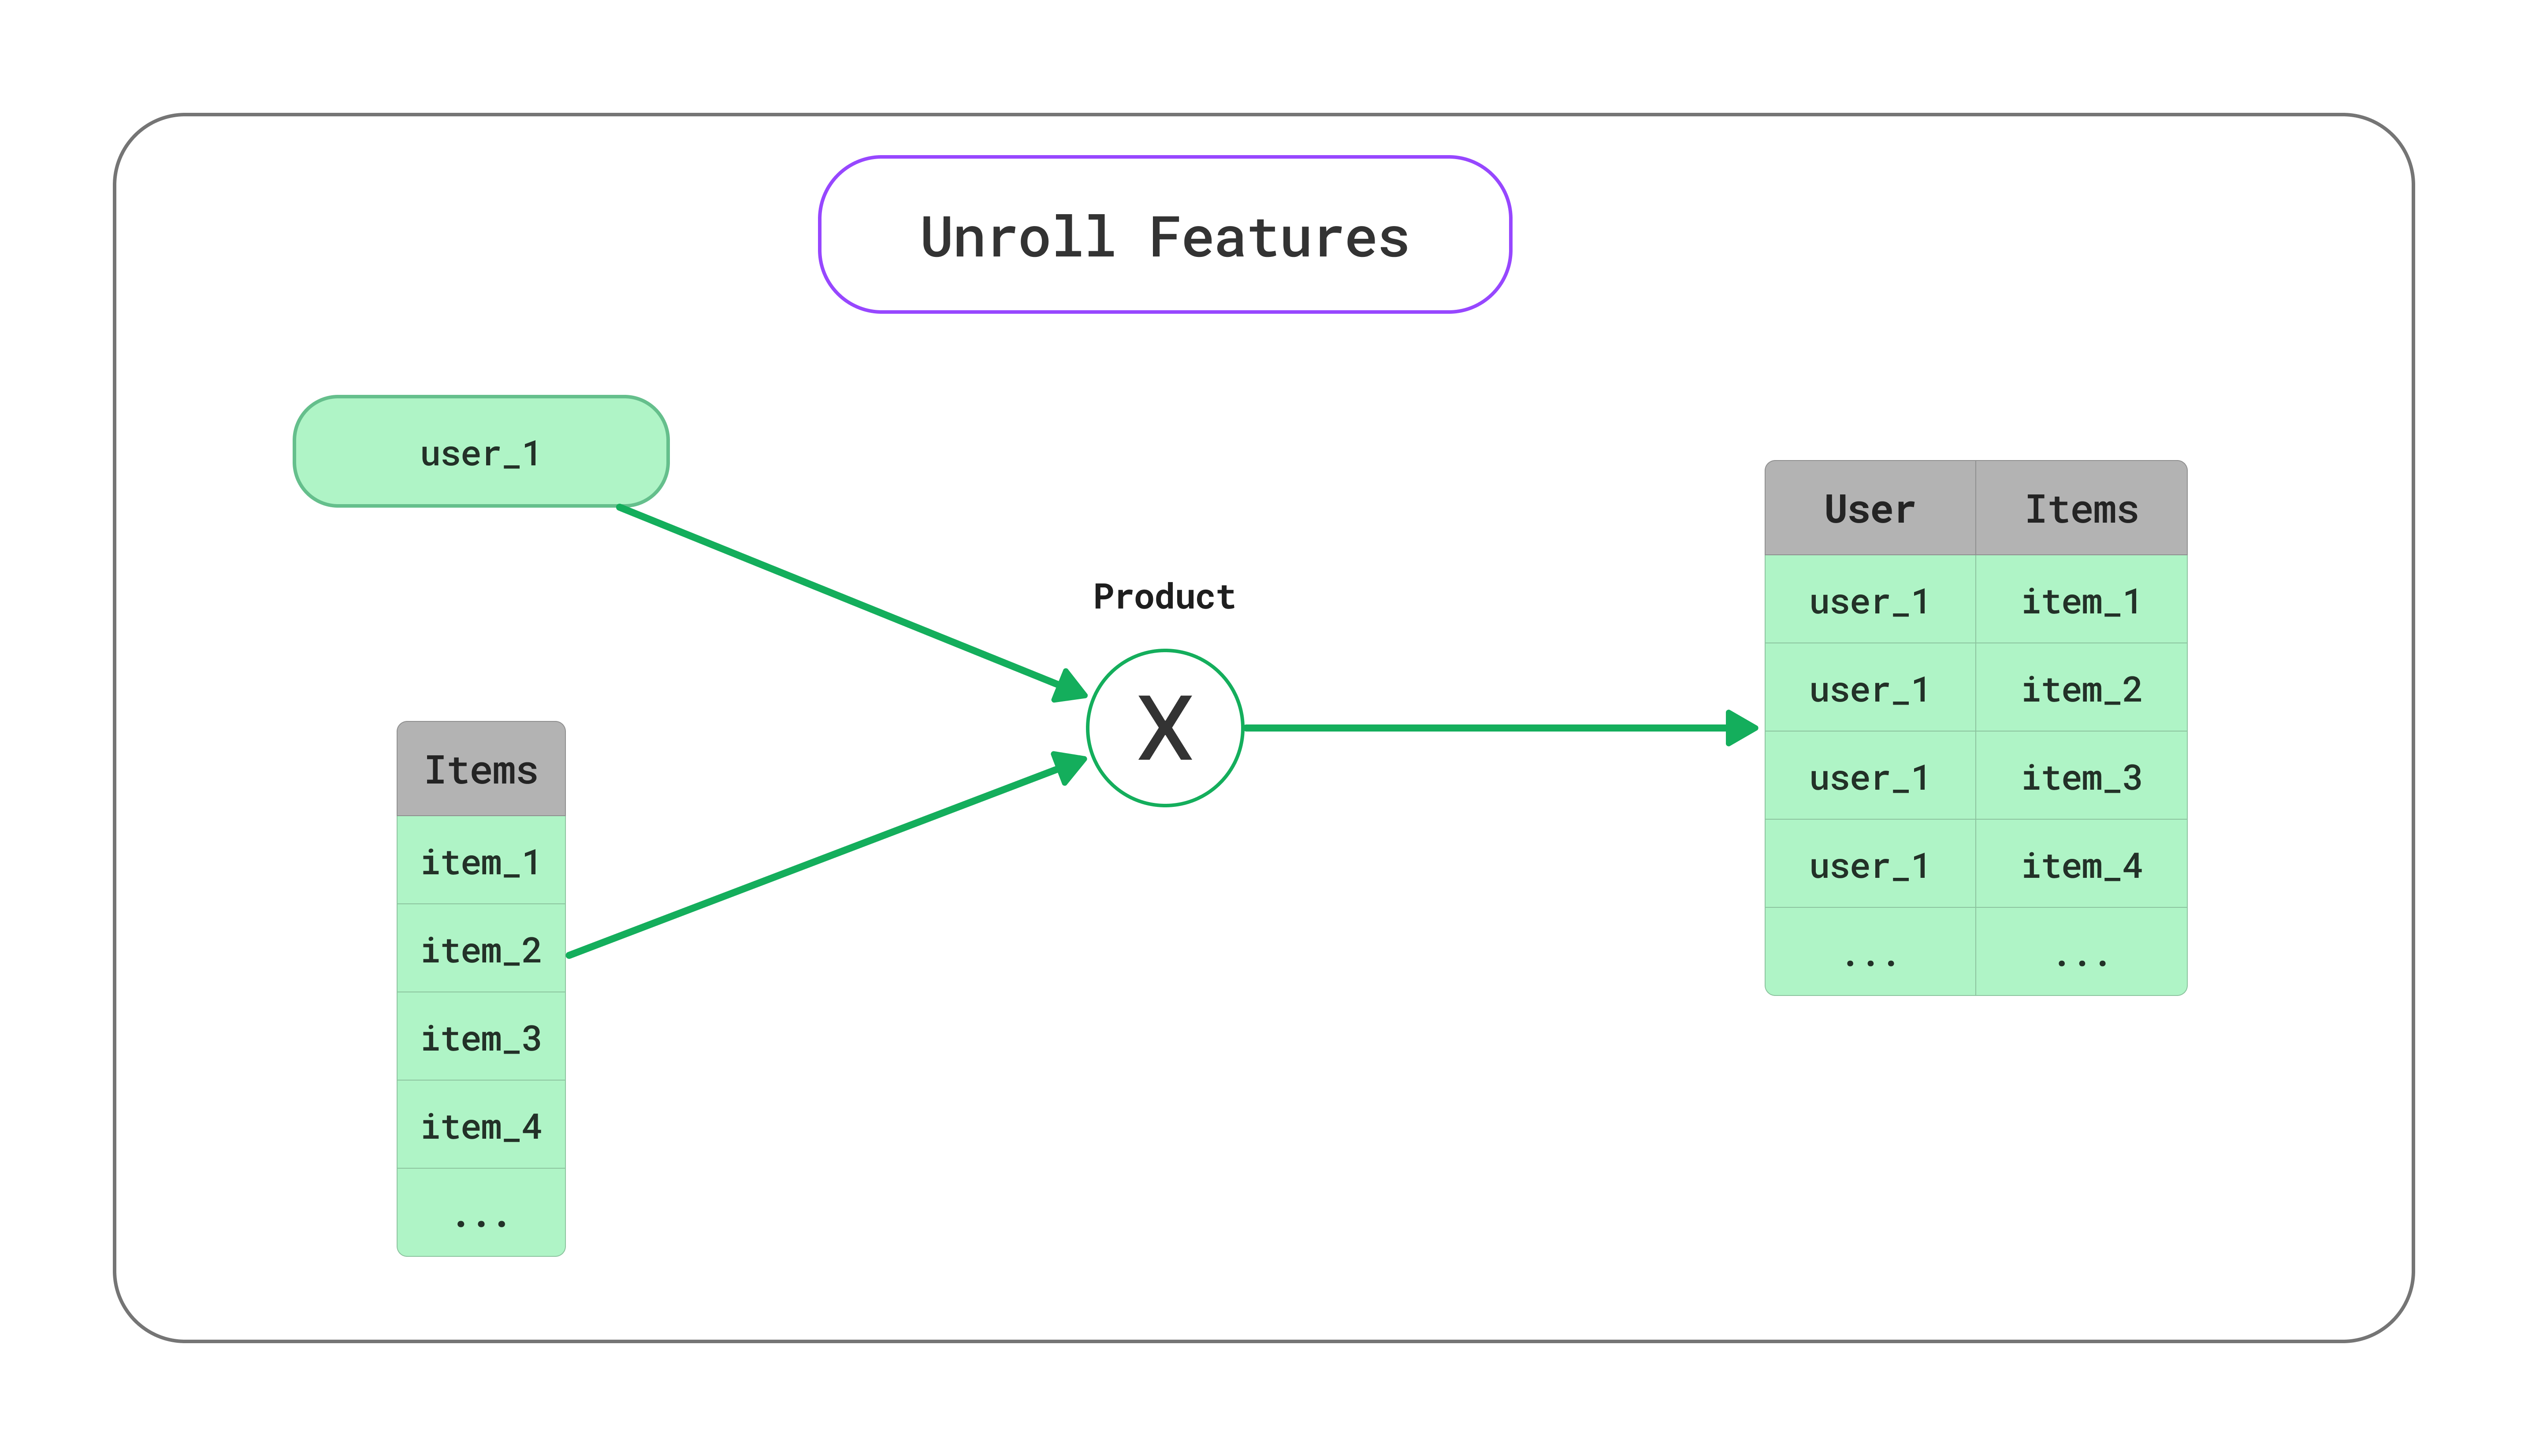
\includegraphics[width=\textwidth]{assets/Unroll Features.png}
    \caption{Unroll User/Item Features}
    \label{fig: UnrollUserFeatures}
\end{figure}


\subsubsection{Score Items}

The server uses the combined user and item features to score each item in the candidate list.
It loads the scoring model, which is responsible for predicting the relevance scores of each item.
The DLRM model is loaded from the model repository using TensorFlow, then the server feeds the combined features into the model to get the relevance scores.
This step outputs a list of item IDs and their corresponding relevance scores (click probability).

\subsubsection{Order Items And Softmax Sampling}

Finally, the server uses the relevance scores to rank the items in the candidate list. 
But instead of returning the top N items, the server uses a softmax sampling technique to sample items from different positions in the ranked list.
The sampling is important to ensure diversity in the recommendations and to avoid recommending the same items to all users or the same items to the same user in different sessions.
In addition, sampling helps the user explore new categories of items and interact with them which tells the system more about the user preferences.
